\documentclass{article}
\setlength{\parskip}{0pt} % esp. entre parrafos
\setlength{\parindent}{20pt} % esp. al inicio de un parrafo
\usepackage{amsmath} % mates
\usepackage{listings}
\usepackage{xcolor}
\usepackage[sort&compress,numbers]{natbib} % referencias
\usepackage{url} % que las URLs se vean lindos
\usepackage[top=10mm,left=20mm,right=20mm,bottom=25mm]{geometry} % \textbf{\textbf{}}margenes
\usepackage{hyperref} % ligas de URLs
\usepackage{graphicx} % poner figuras
\usepackage{caption}
\usepackage{subcaption}
\usepackage[spanish]{babel} % otros idiomas
\hypersetup{
    colorlinks=true,
    linkcolor=blue,
    filecolor=blue,      
    urlcolor=blue,
}
\renewcommand{\lstlistingname}{Código}
\definecolor{codeblack}{rgb}{0,0.6,0}
\definecolor{codegray}{rgb}{0.5,0.5,0.5}
\definecolor{codepurple}{rgb}{0.58,0,0.82}
\definecolor{backcolour}{rgb}{0.95,0.95,0.92}
\lstdefinestyle{mystyle}{
    backgroundcolor=\color{backcolour},   
    commentstyle=\color{codeblack},
    keywordstyle=\color{blue},
    numberstyle=\tiny\color{codegray},
    stringstyle=\color{codeblack},
    basicstyle=\ttfamily\footnotesize,
    breakatwhitespace=false,         
    breaklines=true,                 
    keepspaces=true,                 
    numbers=left,                    
    numbersep=5pt,                  
    showspaces=false,                
    showstringspaces=false,
    showtabs=false,                  
    tabsize=2
}
\lstset{style=mystyle}

\title{"P10" Algoritmo genético}
\author{NESTOR}
\date {Mayo 2022}

\begin{document}

\maketitle

\section{Objetivo}\label{obj}
El objetivo de la práctica consiste en el problema de la mochila (inglés: knapsack) es un problema clásico de optimización, particularmente de programación entera, donde la tarea consiste en seleccionar un subconjunto de objetos de tal forma que (i) no se exceda la capacidad de la mochila en términos de la suma de los pesos de los objetos incluidos, y que (ii) el valor total de los objetos incluidos sea lo máximo posible \cite{elisa1}.

\section{Desarrollo}\label{des}
Basandome en el desarrollo en la \href{https://github.com/satuelisa/Simulation/blob/master/Particles/creation.py}{codificación} implementado por E. Schaeffer y todas las instrucciones se encuentran en el  \href{https://github.com/NestorZeus/SIMULACION-COMPUTACIONAL-DE-NANOMATERIALES/tree/main/P9}{repositorio} de N. Rodríguez en GitHub.\\

Para comenzar se hace primero generar la función para generar partículas de atracción y repulsión con esto para poder visualizar la masa

\begin{lstlisting} [caption=Algoritmo de la combinación óptima., label=codigo2, language=Python]
import math
from scipy.stats import expon
from time import time
def knapsack(peso_permitido, pesos, valores):
    assert len(pesos) == len(valores)
    peso_total = sum(pesos)
    valor_total = sum(valores)
    if peso_total < peso_permitido: 
\end{lstlisting}

Generamos las posiciones de los pesos y valores de las instancias con esto de $1$ a $3$.

\begin{lstlisting}[caption=Pesos y Valores, label=codigo2, language=Python]
def pesos(cuantos, low, high):
    return np.round(normalizar(np.random.uniform(size = cuantos)) * (high - low) + low)
 
def valores(pesos, low, high):
    n = len(pesos)
    valores = np.empty((n))
    for i in range(n):
        valores[i] = np.random.uniform(pesos[i], random(), 1)
    return normalizar(valores) * (high - low) + low
\end{lstlisting}

Para las instancias se crean $n = 40$ con los valores y pesos, a continuación se muestra la codificación:
\begin{lstlisting}[caption=Parámetro de $n$, label=codigo2, language=Python]
n = 40
VP=[]
Tr=[]
for regla in range(3):
    print("############## regla:",regla,"#################")
    if regla == 0:
        pesos = pesos1(n, 23, 100)
        valores = valores1(pesos, 5, 700)
    if regla == 1:
        valores = valores2(n, 5, 700)
        pesos = pesos2(valores, 23, 80)
\end{lstlisting}

Se hace la combinacion de valores y pesos para poder hacer las variaciones de mutaciones, reproducciones y la población. Con esto se genera las replicas e iteracciones.

\begin{lstlisting}[caption=Generacion de funciones, label=codigo2, language=Python]
for pm, init, rep in instancias:
        antesi=time()
        print("#############",pm, init, rep,"#############")
        replicas=3
        best=[]
        porc_dif=[]
        for K in range(replicas):
            p = poblacion_inicial(n, init)
            tam = p.shape[0]
            assert tam == init
            tmax = 100
            mejor = None
            mejores = []
            for t in range(tmax):
                for i in range(tam): # mutarse con probabilidad pm
                    if random() < pm:
                        p = np.vstack([p, mutacion(p[i], n)])
                for i in range(rep):  # reproducciones
                    padres = sample(range(tam), 2)
                    hijos = reproduccion(p[padres[0]], p[padres[1]], n)
                    p = np.vstack([p, hijos[0], hijos[1]])
                tam = p.shape[0]
                d = []
                for i in range(tam):
                    d.append({'idx': i, 'obj': objetivo(p[i], valores),
                              'fact': factible(p[i], pesos, capacidad)})
                d = pd.DataFrame(d).sort_values(by = ['fact', 'obj'], ascending = False)
                mantener = np.array(d.idx[:init])
                p = p[mantener, :]
                tam = p.shape[0]
                assert tam == init
                factibles = d.loc[d.fact == True,]
                mejor = max(factibles.obj)
                mejores.append(mejor)
            best.append(mejor)
            porc_dif.append(((optimo - mejor) / optimo)*100)
        CB.append(porc_dif)
        Ti.append(time()-antesi)
VP.append(CB)
Tr.append(Ti)
\end{lstlisting}

\section{Resultados}\label{res}
\begin{table}[h!]
    \centering
    \caption{Análisis de las instancias}
        \begin{tabular}{|r|r|r|r||r|r||r|r|r|r||r|r|}
    \hline
       Suma de los pesos de los objetos & Mediciones & Estadística\\
       \hline\hline
       Instancia $1$ & $0.09$ & $2.997885194550087$ porciento \\
        \hline
         & $0.20$ & $7.857709388825363$ porciento \\
        \hline
         & $1.0$ & $5.923737554493455$ porciento \\
        \hline
        Instancia $2$ & $23$ & $1.2345504465635582$ porciento \\
        \hline
         & $100$ & $3.0208706337084634$ porciento\\
        \hline
         & $40$ & $0.4934503866186409$ porciento \\
        \hline
        Instancia $3$ & $1.0$ & $0.16747628028044556$ porciento \\
        \hline
         & $900$ & $5.974668588789195$ porciento \\
        \hline
         & $80$ & $3.0175308723987713$ porciento \\
        \hline
    \end{tabular}
    \label{medir_R}
\end{table}

\begin{figure}
    \centering
    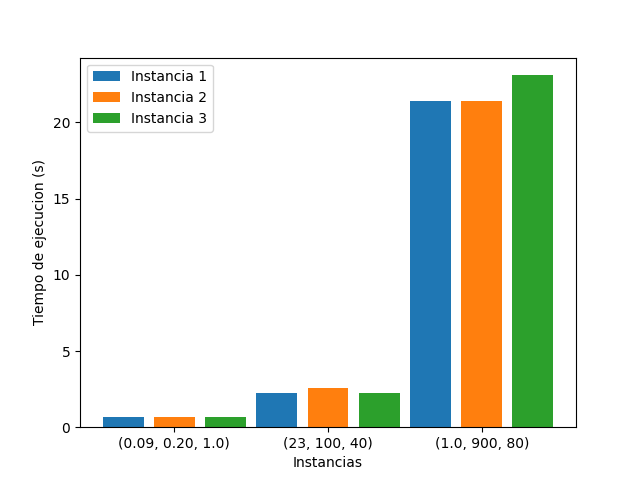
\includegraphics[width=195mm]{Figure_1.png}
    \caption{Analisis de los datos multivariados de las instancias.}
    \label{figure}
\end{figure}

\newpage
\section{Conclusiones}\label{}
Como se puede apreciar en el diagrama de araña que es una herramienta muy útil para mostrar visualmente los gaps entre el estado actual y el estado ideal, se concluye que se puede implementar un algoritmo de genes para poder ejecutar problemas de complejidad en los análisis estadísticos como se observó en el cuadro de análisis de instancias ya que se varía los parámetros y con esto puede llegar a ser el valor óptimo por los valores que se pueden ejecutar con mayor fluidez.

\bibliographystyle{plainnat}
\bibliography{simulacion}
\cite{nestor1}
\cite{elisa1}
\end{document}
